\section{Introduction}

{\color{red}{Proposed story: 1) ML is a data management problem  2) building models is highly iterative  3) data often coming from logs/sensors, that can be faulty  4) faulty datasources means data is dirty, can affect model 5) data prep/cleaning the inputs is hard, lack of tools to do it.  6) coupled with iterative nature (look for problems, clean some, repeat), process is WRONG.  7) Looking at trends such as deep learning, which is very high dimensional, data cleaning is very important, because models are highly sensitivy 8) want an iterative data prep system targeting ML applications 9) ActiveClean is such a system 10) demo on higgs and video.}}


Building distributed frameworks to facilitate model training on large and growing datasets is a key data management challenge with significant interest in both industry and academia~\cite{bdas, alexandrov2014stratosphere, crotty2014tupleware, tensor}.
While these frameworks abstract much of the difficult details of distributed Machine Learning (ML), they seldom offer the analyst any support in terms of constructing the model itself, i.e., which features to use, how to clean the data, and how to evaluate the results.
Data often arrive \emph{dirty}, including missing, incorrect, or inconsistent attributes, and analysts widely report that data cleaning and other forms of pre-processing account for up to 80\% of their effort~\cite{nytimes, kandel2012}.
While data cleaning is an extensively studied problem, the high dimensionality of many models can amplify even a small amount of erroneous records~\cite{xiaofeature}, and the relative complexity (in comparison to SQL analytics) can make it difficult to trace the consequnces of an error.

\begin{figure}[t]
\centering
 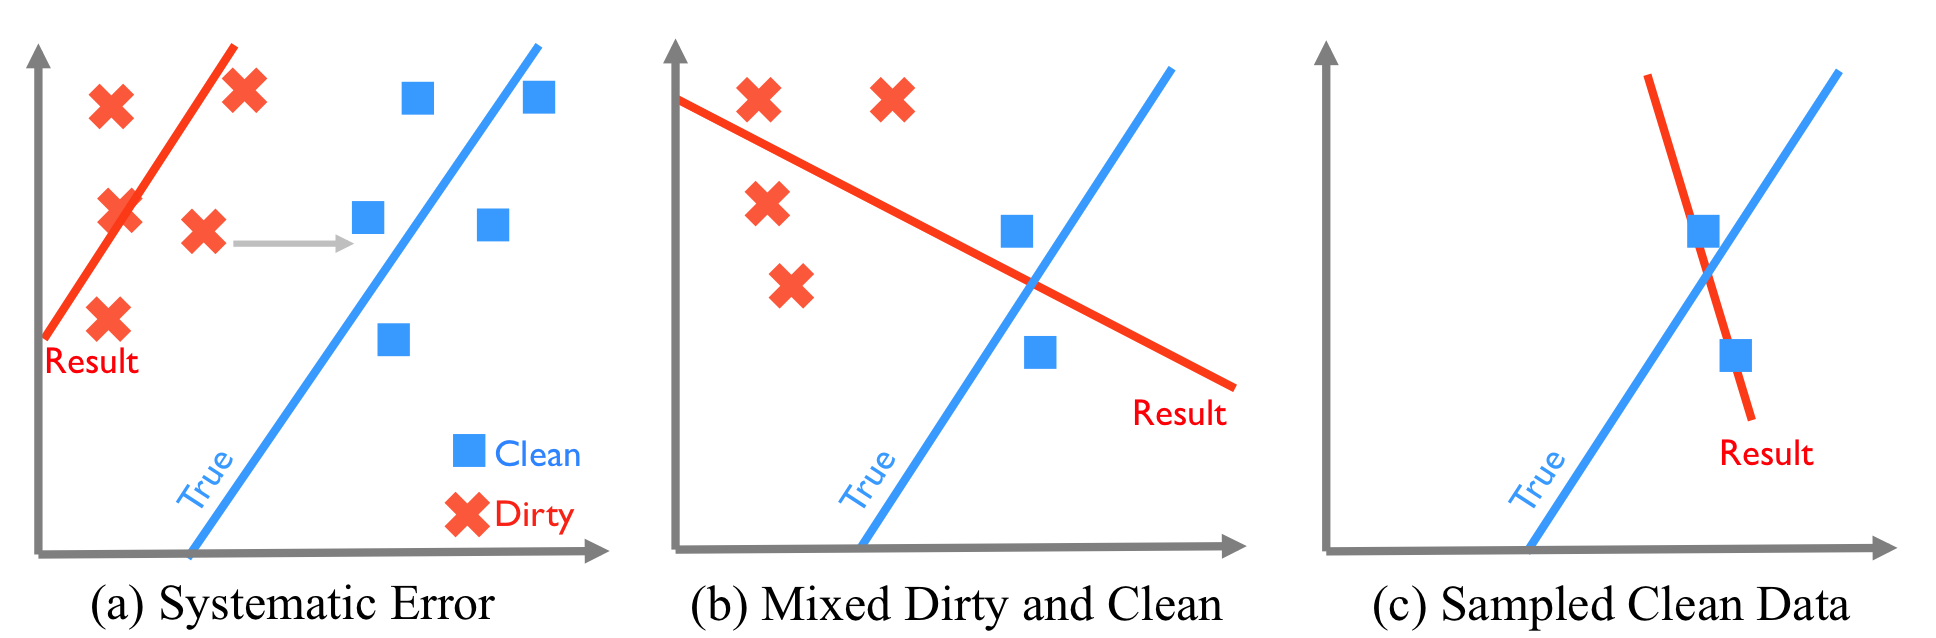
\includegraphics[width=\columnwidth]{figs/update-arch.png}
 \caption{(a) Systematic corruption in one variable can lead to a shifted model. 
 (b) Mixed dirty and clean data results in a less accurate model than no cleaning.
(c) Small samples of only clean data can result in similarly inaccurate models. \label{update-arch1}}
\end{figure}

Consequently, in prior work, we have noted the choice of data cleaning algorithm can significantly affect results even when using robust ML techniques \cite{activecleanarxiv, DBLP:conf/case/MahlerKLSMKPWFAG14}.
In one fraud prediction example, we found that simply applying Entity Resolution before model training improved true positive detection probabilities from 62\% to 91\%. 
Despite this importance, in theory and in practice, the academic community has decoupled the data cleaning problem from featurization and ML.
This is problematic because many ML techniques often make assumptions about data homogeneity and the consistency of sampling, which can be easily violated if the analyst applies data cleaning in an arbitrary way.

To understand how this may happen, consider an anlyst training a regression model on dirty data. At first, she may not realize that there are outliers and train an initial model directly on the dirty data. As she starts to inspect the model, she may realize that some records have a large residual value (not predicted accurately). Once she confirms that those records are indeed dirty, she has to design data cleaning rules or scripts to fix or remove the offending records. After cleaning, she re-trains the model--iterating until she no longer finds dirty data.
This iterative process is the de facto standard, and in fact encouraged by the design of the increasingly popular interactive ``notebook" ML development environments (e.g., IPython), but makes the implicit assumption that model training commutes with incremental data cleaning.
This assumption is wholly incorrect; due to the well-known Simpson's paradox, models trained on a mix of dirty and clean data can have very misleading results even in simple scenarios (Figure \ref{update-arch1}).

In a parallel trend, the dimensionality of the features used in ML models is also rapidly increasing. 
It is now common to use 100,000s of features in image processing processing problems with techniques such as Deep Learning.
Empirically, such feature spaces have facilitated breakthroughs in previously hard classification tasks such as image classification, robot actuation, and speech recognition.
However, the pitfall is that the standard approaches for debugging and reasoning about data error may lose their intuition for higher dimensions.
In other words, it is often not obvious how an analyst should select which records to clean.

As it stands, there are two key problems in interactive model construction, (1) correctness, and (2) dirty data identification.
We address these to problems in a system called \sys which facilitates interactive training-cleaning iteration in a safe way (with expected monotone convergence guarantees) and automatically selects the most valuable data for the analyst to inspect.
\sys is implemented as a Python middleware library that connects IPython notebooks to the Berkeley Data Analytics Stack (BDAS).
The analyst initializes an \sys with an ML model, a featurization function, and the base data, and the \sys initially returns the model trained on the dataset.
\sys also returns an array of data sampled from the model that are possibly dirty.
The analyst can apply any value transformations to the data and then prompt the system to iterate. 
As the analyst cleans more data, \sys learns a internal model to predict which data are likely dirty.

In our demonstration, we will present two experimental datasets: a classification model on the Higgs Boson particle physics dataset (11M records 28 features) and a regression model in a surgical robotics video dataset (50k examples 500000 features).
These datasets are dirty containing outliers and other artifacts of data acquisition.
Participants will be able to use an IPython interface to design and iterate on the model, which will be trained on a cluster using BDAS.
 









